\documentclass[../psets.tex]{subfiles}

\pagestyle{main}
\renewcommand{\leftmark}{Problem Set \thesection}
\stepcounter{section}

\begin{document}




\section{Molecular Spectroscopy}
\begin{enumerate}
    \item \marginnote{3/3:}You propose that you have made a terminal amide (\ce{NH2}) complex. You observe two stretching frequencies in the IR spectrum at \SI{2400}{\per\centi\meter} and \SI{2330}{\per\centi\meter}.
    \begin{enumerate}
        \item Do you have one or two complexes? Rationalize this based on symmetry.
        \begin{proof}[Answer]
            \fbox{One} complex. The two bands correspond to a symmetric and an asymmetric bending mode\footnote{Not a stretch according to Dr. Anderson.} of the same compound.
        \end{proof}
        \item If you deuterate this complex, where should the \ce{N-D} stretches come?
        \begin{proof}[Answer]
            Let
            \begin{align*}
                \nu_{1,\ce{H}} &= \SI{2400}{\per\centi\meter}&
                \nu_{2,\ce{H}} &= \SI{2330}{\per\centi\meter}
            \end{align*}
            We have that
            \begin{align*}
                \mu_{\ce{NH}} &= \frac{m_{\ce{N}}m_{\ce{H}}}{m_{\ce{N}}+m_{\ce{H}}}
                    = \frac{14\cdot 1}{14+1}
                    = 0.933&
                \mu_{\ce{ND}} &= \frac{m_{\ce{N}}m_{\ce{D}}}{m_{\ce{N}}+m_{\ce{D}}}
                    = \frac{14\cdot 2}{14+2}
                    = 1.75
            \end{align*}
            Thus,
            \begin{align*}
                \nu_{1,\ce{D}} &= \frac{\sqrt{\mu_{\ce{NH}}}}{\sqrt{\mu_{\ce{ND}}}}\cdot\nu_{1,\ce{H}}&
                \nu_{2,\ce{D}} &= \frac{\sqrt{\mu_{\ce{NH}}}}{\sqrt{\mu_{\ce{ND}}}}\cdot\nu_{2,\ce{H}}
            \end{align*}
            Plugging in numbers, we learn that
            \begin{empheq}[box=\fbox]{align*}
                \nu_{1,\ce{D}} &= \SI{1750}{\per\centi\meter}&
                \nu_{2,\ce{D}} &= \SI{1700}{\per\centi\meter}
            \end{empheq}
        \end{proof}
    \end{enumerate}
    \item Copper (II) acetate is a dimer and the two \ce{Cu} atoms strongly interact. The EPR spectrum consists of seven lines with intensities of $1:2:3:4:3:2:1$. Copper nuclei have $I=3/2$, and copper acetate consists of a ground state singlet with an accessible triplet excited state. Explain the number and relative intensity of the observed signals.
    \begin{proof}[Answer]
        % Multiline patterns: $2nI+1=2\cdot 2\cdot 3/2+1=7$ lines.
        % Sum the contributions from other neighboring nuclei.

        % Would one electron feel the same contribution from both nuclei since it's orbiting around them in a delocalized fashion? Would it be because what's felt is the net $M_I$.

        % We add the $M_I$'s of the component nuclei to have our second splitting run $-3,-2,\dots,3$. There's seven allowed peaks.


        Since there are $n=2$ copper atoms each with nuclear spin $I=3/2$, then $2nI+1$ rule predicts that there will be
        \begin{equation*}
            2\cdot 2\cdot\frac{3}{2}+1 = 7
        \end{equation*}
        lines in the spectrum. As to the relative intensities, since the $M_I$ contributions from all relevant nuclei sum, we know that overall, $I=3/2$ and $M_I=-3,-2,\dots,3$ (i.e., can take on \emph{seven} values, again as predicted by the $2nI+1$ rule). Additionally, we can identify the number of microstates that can yield each value of $M_I$. For instance, $-3$ must be the sum of $(-3/2)+(-3/2)$. However,
        \begin{equation*}
            -2 = (-3/2)+(-1/2)=(-1/2)+(-3/2)
        \end{equation*}
        so there are \emph{two} microstates that correspond to it. Continuing on, we can determine that the quantum number $M_I$ corresponds to $M_I+4$ microstates. Additionally, the transition energies will grow as $M_I$ increases (according to the relevant triplet hyperfine splitting diagram), meaning that the peak splitting pattern
        \begin{equation*}
            1:2:3:4:3:2:1
        \end{equation*}
        will indeed be realized as quantum number (and hence energy) varies from lesser to greater.
    \end{proof}
    \item The intensities and frequencies (vs. \ce{H3PO4}) of resonances in the \SI{121.4}{\mega\hertz} \ce{{}^31P}\{\ce{{}^1H}\} NMR spectrum of \ce{Pt(PPh3)\{\eta^3-N(CH2CH2PPh2)3\}} are listed below. Determine the chemical shifts (i.e., $\delta$ values) and coupling constants, and draw the structure.
    \begin{center}
        \small
        \renewcommand{\arraystretch}{1.2}
        \begin{tabular}{SSS}
            \textbf{Frequency} & \textbf{Intensity} & \textbf{Chemical shift}\\
            \hline
            -3393.4 & 7.8  & \color{blx}-27.95\\
            -3313.5 & 7.7  & \color{blx}-27.29\\
            -1484.8 & 31.1 & \color{blx}-12.23\\
            -1404.9 & 31.3 & \color{blx}-11.57\\
            -833.3  & 0.7  & \color{blx}-6.864\\
            -753.5  & 1.9  & \color{blx}-6.207\\
            -673.4  & 2.0  & \color{blx}-5.547\\
            -593.6  & 0.6  & \color{blx}-4.890\\
            263.7   & 7.9  & \color{blx}2.172\\
            343.7   & 7.7  & \color{blx}2.831\\
            1385.5  & 2.6  & \color{blx}11.41\\
            1465.6  & 7.8  & \color{blx}12.07\\
            1545.8  & 7.6  & \color{blx}12.73\\
            1625.6  & 2.7  & \color{blx}13.39\\
            3604.5  & 0.7  & \color{blx}29.69\\
            3684.6  & 1.9  & \color{blx}30.35\\
            3764.4  & 1.9  & \color{blx}31.01\\
            3844.7  & 0.6  & \color{blx}31.67\\
        \end{tabular}
    \end{center}
    \begin{proof}[Answer]
        % Confirm chemical shift formula: Times \num{e6}, not divided by??

        % Coupling constant: So for adjacent nuclei, subtract the frequencies and then convert to chemical shift??


        To convert to chemical shift (\si{\ppm}), use the formula
        \begin{equation*}
            \frac{\nu_1-\nu_\text{ref}}{\nu_0}\times\num{e6}
        \end{equation*}
        where $\nu_1$ is the measured frequency for a given nucleus, $\nu_\text{ref}=0$ in this case, and $\nu_0=\SI{121.4}{\mega\hertz}$ is the spectrometer frequency. An example calculation for the first row in the given table is shown below.
        \begin{equation*}
            \frac{\SI{-3393.4}{\hertz}-\SI{0}{\hertz}}{\SI{121.4}{\mega\hertz}}\times\num{e6} = \frac{\SI{-3393.4}{\hertz}}{\SI{121.4}{\hertz}}
            = \SI{-27.95}{\ppm}
        \end{equation*}
        The rest of the results are tabulated above in blue.
        There are six peaks present in the spectrum. The coupling constant of each peak is either equal to the peak splitting, or the average of the three peak splittings in the case of the three quartets present. For example, the coupling constant for the peak centered around \SI{-27.62}{\ppm} is
        \begin{equation*}
            J_1 = (\SI{-27.29}{\ppm})-(\SI{-27.95}{\ppm}) = \SI{0.66}{\ppm}
        \end{equation*}
        and the coupling constant for the peak centered around \SI{-5.877}{\ppm} is
        \begin{align*}
            J_3 &= \frac{[(\SI{-4.890}{\ppm})-(\SI{-5.547}{\ppm})]+[(\SI{-5.547}{\ppm})-(\SI{-6.207}{\ppm})]+[(\SI{-6.207}{\ppm})-(\SI{-6.864}{\ppm})]}{3}\\
            &= \frac{(\SI{-4.890}{\ppm})-(\SI{-6.864}{\ppm})}{3}\\
            &= \SI{0.658}{\ppm}
        \end{align*}
        Altogether, the coupling constants from lowest \si{\ppm} to highest \si{\ppm} are given by
        \begin{empheq}[box=\fbox]{align*}
            J_1 &= 0.66&
            J_2 &= 0.66&
            J_3 &= 0.658&
            J_4 &= 0.659&
            J_5 &= 0.660&
            J_6 &= 0.660
        \end{empheq}
        where all quantities are in units of ppm.\par
        Lastly, the structure is as follows.
        \begin{center}
            \footnotesize
            \chemfig{Pt(-[:100,,,1]PPh_2-[:175]-[::30]-[::30]N?)(-[:-100,,,1]PPh_2-[:-175]-[::-30]-[::-30]?)(-[:150,,,1]PPh_2-[:175,0.5]-[::30,0.5]?)-PPh_3}
        \end{center}
    \end{proof}
    \item Predict the spin state, $\mu_\text{eff}$, and $\chi T$ values for the following ions in the indicated geometry.
    \begin{enumerate}
        \item Tetrahedral \ce{Mn(II)}.
        \begin{proof}[Answer]
            % Do octahedral and tetrahedral affect high spin/low spin in your approximation, or just oxidation state? Can square planar ever be high spin?

            % Row (second-third LS), then geometry dominates, then oxidation state.


            As a first-row transition metal with $T_d$ geometry, \ce{Mn(II)} will be \fbox{high spin.} It follows that as a $d^5$ metal center, \ce{Mn(II)} will have 5 unpaired electrons. Thus,
            \begin{align*}
                \mu_\text{eff} &= \sqrt{4\left( \frac{5}{2}\left( \frac{5}{2}+1 \right) \right)}&
                    \chi T &= \frac{1}{2}\left( \frac{5}{2}\left( \frac{5}{2}+1 \right) \right)\\
                \Aboxed{\mu_\text{eff} &= 5.92}&
                    \Aboxed{\chi T &= 4.375}
            \end{align*}
        \end{proof}
        \item Octahedral \ce{Ir(III)}.
        \begin{proof}[Answer]
            As a third-row transition metal, \ce{Ir(III)} will be \fbox{low spin.} It follows that as a $d^6$ metal center, \ce{Ir(III)} will have 0 unpaired electrons. Thus,
            \begin{align*}
                \mu_\text{eff} &= \sqrt{4\left( \frac{0}{2}\left( \frac{0}{2}+1 \right) \right)}&
                    \chi T &= \frac{1}{2}\left( \frac{0}{2}\left( \frac{0}{2}+1 \right) \right)\\
                \Aboxed{\mu_\text{eff} &= 0}&
                    \Aboxed{\chi T &= 0}
            \end{align*}
        \end{proof}
        \item Octahedral \ce{Ru(III)}.
        \begin{proof}[Answer]
            As a second-row transition metal, \ce{Ru(III)} will be \fbox{low spin.} It follows that as a $d^5$ metal center with $O_h$ geometry, \ce{Ru(III)} will have 1 unpaired electron. Thus,
            \begin{align*}
                \mu_\text{eff} &= \sqrt{4\left( \frac{1}{2}\left( \frac{1}{2}+1 \right) \right)}&
                    \chi T &= \frac{1}{2}\left( \frac{1}{2}\left( \frac{1}{2}+1 \right) \right)\\
                \Aboxed{\mu_\text{eff} &= 1.73}&
                    \Aboxed{\chi T &= 0.375}
            \end{align*}
        \end{proof}
        \item Square planar \ce{Co(I)}.
        \begin{proof}[Answer]
            As a square planar complex, \ce{Co(I)} will be \fbox{low spin.} It follows that as a $d^8$ metal center with $D_{4h}$ geometry, \ce{Co(I)} will have 0 unpaired electron. Thus,
            \begin{align*}
                \mu_\text{eff} &= \sqrt{4\left( \frac{0}{2}\left( \frac{0}{2}+1 \right) \right)}&
                    \chi T &= \frac{1}{2}\left( \frac{0}{2}\left( \frac{0}{2}+1 \right) \right)\\
                \Aboxed{\mu_\text{eff} &= 0}&
                    \Aboxed{\chi T &= 0}
            \end{align*}
        \end{proof}
        \item Square planar \ce{Pt(II)}.
        \begin{proof}[Answer]
            As a third-row transition metal, \ce{Pt(II)} will be \fbox{low spin.} It follows that as a $d^8$ metal center with $D_{4h}$ geometry, \ce{Pt(II)} will have 0 unpaired electron. Thus,
            \begin{align*}
                \mu_\text{eff} &= \sqrt{4\left( \frac{0}{2}\left( \frac{0}{2}+1 \right) \right)}&
                    \chi T &= \frac{1}{2}\left( \frac{0}{2}\left( \frac{0}{2}+1 \right) \right)\\
                \Aboxed{\mu_\text{eff} &= 0}&
                    \Aboxed{\chi T &= 0}
            \end{align*}
        \end{proof}
        \item Octahedral \ce{Ni(II)}.
        \begin{proof}[Answer]
            As a first-row transition metal with $O_h$ geometry, \ce{Ni(II)} will be \fbox{low spin.} It follows that as a $d^8$ metal center, \ce{Ni(II)} will have 2 unpaired electrons. Thus,
            \begin{align*}
                \mu_\text{eff} &= \sqrt{4\left( \frac{2}{2}\left( \frac{2}{2}+1 \right) \right)}&
                    \chi T &= \frac{1}{2}\left( \frac{2}{2}\left( \frac{2}{2}+1 \right) \right)\\
                \Aboxed{\mu_\text{eff} &= 2.82}&
                    \Aboxed{\chi T &= 1}
            \end{align*}
        \end{proof}
        \item Tetrahedral \ce{Cr(0)}.
        \begin{proof}[Answer]
            High spin.
            As a first-row transition metal with $T_d$ geometry, \ce{Cr(0)} will be \fbox{high spin.} It follows that as a $d^6$ metal center, \ce{Cr(0)} will have 4 unpaired electrons. Thus,
            \begin{align*}
                \mu_\text{eff} &= \sqrt{4\left( \frac{4}{2}\left( \frac{4}{2}+1 \right) \right)}&
                    \chi T &= \frac{1}{2}\left( \frac{4}{2}\left( \frac{4}{2}+1 \right) \right)\\
                \Aboxed{\mu_\text{eff} &= 4.90}&
                    \Aboxed{\chi T &= 3}
            \end{align*}
        \end{proof}
    \end{enumerate}
    \item Predict whether the following high-spin ions should have an isotropic EPR $g$-value greater than, equal, or less than 2.
    \begin{enumerate}
        \item \ce{Cu(II)}.
        \begin{proof}[Answer]
            % $d^9$, more than half filled, $g>2$.

            % Rationalization: Ring current consists of hopping hole, which reinforces the field, which means that we don't need $H_r$ to be as high in $g=h\nu/\beta H_r$ to achieve the transition. With $H_r$ lower, $g$ is higher.

            \ce{Cu(II)} has a $d^9$ configuration, i.e., its $d$-shell is more than half filled. Thus, by the rule discussed in class,
            \begin{equation*}
                \boxed{g > 2}
            \end{equation*}
            The intuitive (but not quantum mechanically accurate) reason for this is that in a $d^9$ configuration, one \emph{hole} hops around producing a ring current that \emph{reinforces} the magnetic field, which means that we don't need $H_r$ to be as high in $g=h\nu/\beta H_r$ to achieve the transition. With $H_r$ lower, $g$ is higher.
        \end{proof}
        \item \ce{Cr(V)}.
        \begin{proof}[Answer]
            \ce{Cr(V)} has a $d^1$ configuration, i.e., its $d$-shell is less than half filled. Thus, by the rule discussed in class,
            \begin{equation*}
                \boxed{g < 2}
            \end{equation*}
        \end{proof}
        \pagebreak
        \item \ce{Mn(II)}.
        \begin{proof}[Answer]
            \ce{Mn(II)} has a $d^5$ configuration, i.e., its $d$-shell is exactly half filled. Thus, by the rule discussed in class,
            \begin{equation*}
                \boxed{g \approx 2}
            \end{equation*}
        \end{proof}
        \item \ce{Fe(III)}.
        \begin{proof}[Answer]
            \ce{Fe(III)} has a $d^5$ configuration, i.e., its $d$-shell is exactly half filled. Thus, by the rule discussed in class,
            \begin{equation*}
                \boxed{g \approx 2}
            \end{equation*}
        \end{proof}
        \item \ce{Co(II)}.
        \begin{proof}[Answer]
            \ce{Co(II)} has a $d^7$ configuration, i.e., its $d$-shell is more than half filled. Thus, by the rule discussed in class,
            \begin{equation*}
                \boxed{g > 2}
            \end{equation*}
        \end{proof}
    \end{enumerate}
    \item If you were handed two vials, one with ferrocene and one with ferrocenium, how could you use XAS and Mossbauer to determine which was which?
    \begin{proof}[Answer]
        In XAS, varying oxidation states shift the $K$-edge. In particular, since ferrocenium has a more highly oxidized iron atom, \ce{Fe} will hold onto its electrons more tightly, shifting its $K$-edge higher.\par
        In Mossbauer, a higher oxidation states mean less electron density at the nucleus. Thus, the $\gamma$ ray would not need to be as high intensity to pierce through the surrounding electron cloud, meaning that the the isomer shift will be lower for ferrocenium.
    \end{proof}
    \item 
    \begin{enumerate}
        \item Name 3 pieces of structural information you can get from a $K$-edge EXAFS spectrum on an unknown TM complex with at least one phosphine ligand.
        \begin{proof}[Answer]
            % The effect of the phosphine ligand??

            You can obtain the \fbox{number} of adjacent scatterers (including phosphine ligands), some information on the \fbox{type} of scatterers that may help determine what they are, and the \fbox{distance} of scatters, i.e., the bond length.
        \end{proof}
        \item A Mossbauer spectrum of an \ce{FeL5} complex shows two signals with differing isomer shifts and quadrupole splittings. Offer an explanation for this.
        \begin{proof}[Answer]
            % Low spin vs. high spin?? What's going on here?
            % \ce{Fe^{III}} varies from 0.0 to 0.6 based on quadrupole splitting.

            You could have two different isomers, one square pyramidal and one trigonal bipyramidal.
        \end{proof}
    \end{enumerate}
    \item Draw a clearly labeled diagram representing the expected EPR spectrum of an aqueous \ce{{}^63Cu^2+} ion ($I=3/2$) at room temperature. Clearly indicate the position of the isotropic $g$-value.
    \begin{proof}[Answer]
        % Solution makes it isotropic. We'll have 4 peaks. What do you mean by position of $g$?? How does the mass number factor in?
        % Copper (II) is $d^9$.

        Since the $d^9$ (one electron unpaired) ion is in solution (not frozen), the $g$-values will be isotropic. Additionally, $I=3/2$ and the relevant selection rules ($\Delta M_S=\pm 1$ and $\Delta M_I=0$) means that the hyperfine splitting splits the peak into a quartet of peaks with the same height. Thus, the EPR spectrum should resemble the following.
        \begin{center}
            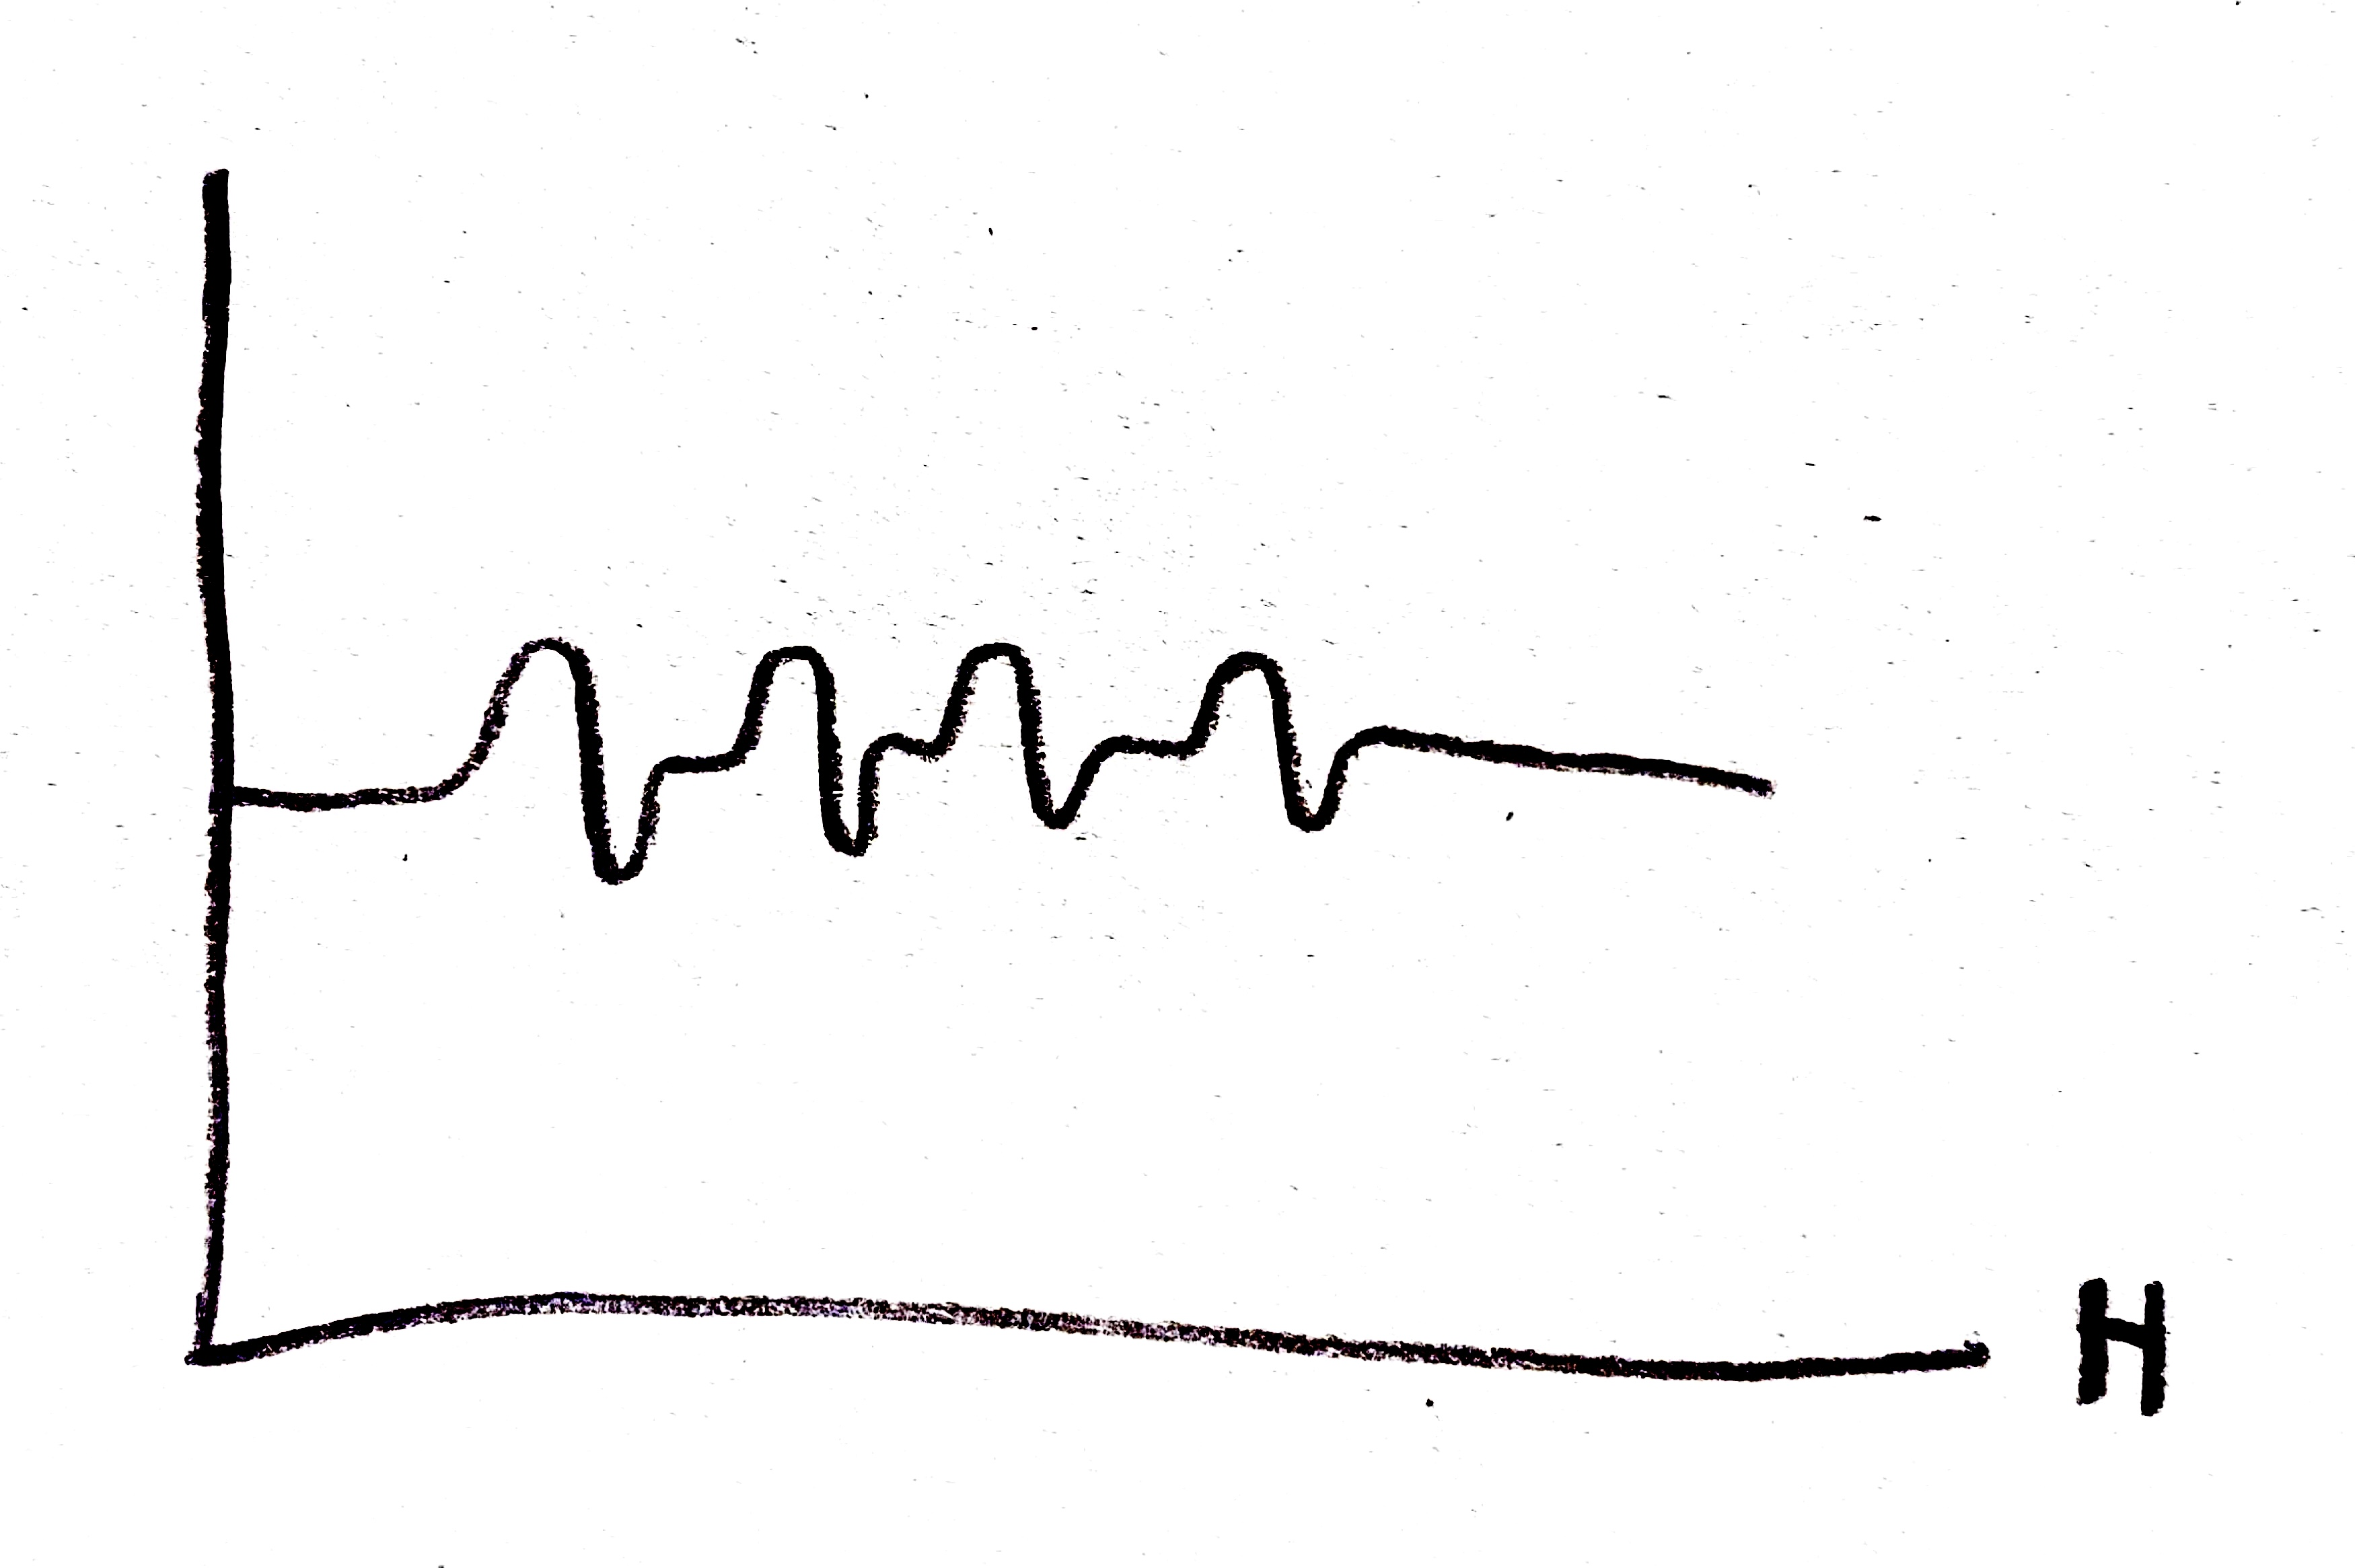
\includegraphics[width=0.4\linewidth]{PSet2-EPR.jpg}
        \end{center}
    \end{proof}
    \item The EPR spectrum of an axially symmetric \ce{Cu^2+} complex in a frozen solution that is 100\% \ce{{}^63Cu} consists of three well-resolved low field $g$-parallel components, a fourth component of the multiplet that overlaps the $g$-perpendicular signal, and some higher field lines. The minima between the four largely resolved components appear at \SI{2720}{\gauss}, \SI{2810}{\gauss}, and \SI{2900}{\gauss}. Given this information and a spectrometer frequency of \SI{9.12}{\giga\hertz}\dots
    \begin{enumerate}
        \item Compute the value of $g_\parallel$;
        \begin{proof}[Answer]
            As stated in the question, the $g_\parallel$ component of the EPR spectrum appears in a quartet with center minimum at \SI{2810}{\gauss}. Thus,
            \begin{align*}
                g &= \frac{h\nu}{\beta H_r}\\
                &= \frac{(\SI{6.626e-34}{\joule\second})(\SI{9.12e9}{\per\second})}{(\SI{9.3e-24}{\joule\per\tesla})(\SI{0.281}{\tesla})}\\
                \Aboxed{g &= 2.32}
            \end{align*}
        \end{proof}
        \item Compute the hyperfine coupling constant.
        \begin{proof}[Answer]
            We have that
            \begin{align*}
                a &= g\beta A\\
                &= (2.32)(\SI{9.3e-24}{\joule\per\tesla})(\SI{0.009}{\tesla})\\
                &= \SI{1}{\joule}
            \end{align*}
        \end{proof}
    \end{enumerate}
    \item The structure of the active site of carbon monoxide dehydrogenase was determined from XAS data to be
    \begin{center}
        \footnotesize
        \chemfig{Mo(-[:30]S-[:-30]Cu-[:30]S-[:-30])(=[2]O)(-[:150]@{S1}S)(-[:-150]@{S2}S)(-[:-30]OH)}
        \chemmove{
            \draw [-,shorten <=3pt,shorten >=3pt] (S1) to[bend right=40] (S2);
        }
    \end{center}
    \begin{enumerate}
        \item Indicate how you could identify the heavy atoms with XANES or EXAFS data, the oxidation state of these atoms, and the coordination environment.
        \begin{proof}[Answer]
            % Heavy atoms by $K$-edge, oxidation state by $K$-edge shift, coordination environment from EXAFS. Detail??

            The heavy atoms can be identified by the $K$-edge energy. The oxidation state can technically be identified by the $K$-edge shift from the standard, although XAS is typically more useful for measuring relative oxidation states than "absolute" ones. The coordination environment can be determined by fitting the EXAFS data to the EXAFS equation.
        \end{proof}
        \item Your results tell you that the oxidation states of \ce{Mo} and \ce{Cu} are $6+$ and $1+$, respectively. How could you determine the protonation state of the hydroxide (\ce{OH} or \ce{OH2}) with ENDOR spectroscopy?
        \begin{proof}[Answer]
            ENDOR turns on extra transitions. Protonation should correlate with the oxidation state, affecting splitting. Since ENDOR allows us to resolve extra transitions and learn more about electron transitions that are coupled to local nuclear transitions, that could also be of use.
        \end{proof}
    \end{enumerate}
    \item For the following fragments, predict the $\chi T$ and $\mu_\text{eff}$ values for anti-ferromagnetic, ferromagnetic, and uncoupled scenarios. Using the indicated room temperature $\chi T$ or $\mu_\text{eff}$ values, predict the coupling in these fragments. Assume no contributions from spin-orbit coupling.
    \begin{enumerate}
        \item \ce{Cu^{II}-X-Cu^{II}}, $\chi T=\SI{0.4}{\centi\meter\cubed\kelvin\per\mole}$.
        \begin{proof}[Answer]
            We take the pythagorean average of the two?? See Lecture 6.2.
        \end{proof}
        \item \ce{Ni^{II}-X-Cr^{II}}, $\chi T=\SI{4.4}{\centi\meter\cubed\kelvin\per\mole}$.
        \begin{proof}[Answer]
            
        \end{proof}
        \item \ce{Fe^{III}-X-Fe^{III}}, $\mu_\text{eff}=8.4\,\mB$.
        \begin{proof}[Answer]
            
        \end{proof}
        \item \ce{Fe^{II}-X-Fe^{III}}, $\chi T=\SI{11}{\centi\meter\cubed\kelvin\per\mole}$.
        \begin{proof}[Answer]
            
        \end{proof}
    \end{enumerate}
    \item You synthesize a series of new metal oxides with each metal center in an $O_h$ coordination environment. The two metals alternate in an edge-sharing \ce{AB}. You note that when $\ce{A}=\ce{Ti(III)}$ and $\ce{B}=\ce{Cu(II)}$, the material exhibits strong ferromagnetic exchange. However, when $\ce{A}=\ce{Fe(III)}$, a strong antiferromagnetic exchange is observed. Rationalize these two observations.
    \begin{proof}[Answer]
        \ce{Ti(III)} is $d^1$ and \ce{Cu(II)} is $d^9$. Thus, each metal center has one unpaired electron, and they are likely to couple parallel, or ferromagnetically. However, when \ce{Fe(III)} is present, we have more of a situation of one hole moving around, and thus antiferromagnetic exchange is more active.
    \end{proof}
\end{enumerate}




\end{document}